\documentclass[a4paper, 11pt]{article}
\usepackage[UTF8]{ctex}
\usepackage{amsmath}
\usepackage{graphicx}
\usepackage{geometry}
\usepackage{listings}
\geometry{scale=0.8}
\linespread{1.5}
\usepackage{hyperref}
\usepackage{listings}

\title{	
\normalfont \normalsize
\textsc{School of Data and Computer Science, Sun Yat-sen University} \\ [25pt] %textsc small capital letters
\rule{\textwidth}{0.5pt} \\[0.4cm] % Thin top horizontal rule
\huge  E06 Queries on KB \\ % The assignment title
\rule{\textwidth}{2pt} \\[0.5cm] % Thick bottom horizontal rule
\author{17341175 徐志成}
\date{\normalsize\today}
}
\lstset{numbers=left, %设置行号位置
        numberstyle=\tiny, %设置行号大小
        keywordstyle=\color{blue}, %设置关键字颜色
        commentstyle=\color[cmyk]{1,0,1,0}, %设置注释颜色
        frame=single, %设置边框格式
        escapeinside=``, %逃逸字符(1左面的键),用于显示中文
        breaklines, %自动折行
        extendedchars=false, %解决代码跨页时,章节标题,页眉等汉字不显示的问题
        xleftmargin=2em,xrightmargin=2em, aboveskip=1em, %设置边距
        tabsize=4, %设置tab空格数
        showspaces=false %不显示空格
       }

\begin{document}
\maketitle
\tableofcontents
\newpage


\section{Problem Description}
Given a KB \texttt{Restaurants.pl}, which describes the distribution of branches of 10 well-known restaurants in Guangzhou. 

For example, \texttt{restaurant(ajukejiacai,2007,yuecai)} means that \texttt{ajukejiacai} was founded in 2007 and is a restaurant of \texttt{yuecai}. \texttt{branch(ajukejiacai,xintiandi)} means that \texttt{ajukejiacai} has a branch in \texttt{xintiandi}. \texttt{district(xintiandi,panyu)} means that \texttt{xintiandi} is an area of \texttt{panyu} district.

Please formulate each of the following questions as a query using Prolog's notation, pose it to Prolog, and obtain Prolog's answer:
\begin{enumerate}
  \item What restaurants have branches in beigang? 
  \item What districts have restaurants of yuecai and xiangcai?
  \item What restaurants have the least number of branches?
  \item What areas have two or more restaurants?
\item Which restaurant has the longest history?
\item What restaurants have at least 10 branches?
\end{enumerate}
Please define the new relation below using Prolog and test it.
\begin{itemize}
\item sameDistrict(Restaurant1, Restaurant2): Restaurant1 and Restaurant2 have one or more branches in the same district.
\end{itemize}




You should write down a listing that shows the queries you submitted to Prolog, and the answer returned. Hand in a file named \textsf{E06\_YourNumber.pdf}, and send it to \textsf{ai\_201901@foxmail.com}


\section{Codes and Results}
\begin{lstlisting}[language=C]
1.setof(A,(branch(A,beigang)),Res).

2.setof(C,((restaurant(A,_,yuecai),branch(A,B),district(B,C),restaurant(D,_,xiangcai),branch(D,F),district(F,C))),Res).

3.setof(A1,(Y^Y2^(setof(B1,branch(A1,B1),Results1),length(Results1,Y),\+ (setof(B2,branch(A2,B2),Results2),length(Results2,Y2),\+ Y=<Y2))),Res).
 % 这里不用Y^Y2 也是可以的,因为prolog 语言中的变量默认是按照存在来寻找的,变量为存在量词,同理5 也是如此
4.setof(B,(setof(A,branch(A,B),Results),length(Results,C),C>=2),Res).
5.setof(A1,(Y^Y2^(restaurant(A1,Y,_),\+ (restaurant(A2,Y2,_),\+ Y=<Y2))),Res).
6.setof(A,(setof(B,branch(A,B),Results),length(Results,C),C>=10),Res).

7.sameDistrict(A,B):-branch(A,C),branch(B,D),C=D,A\=B.
query:findall(pair(A,B),sameDistrict(A,B),Res).
\end{lstlisting}

\begin{figure}[ht]
\centering
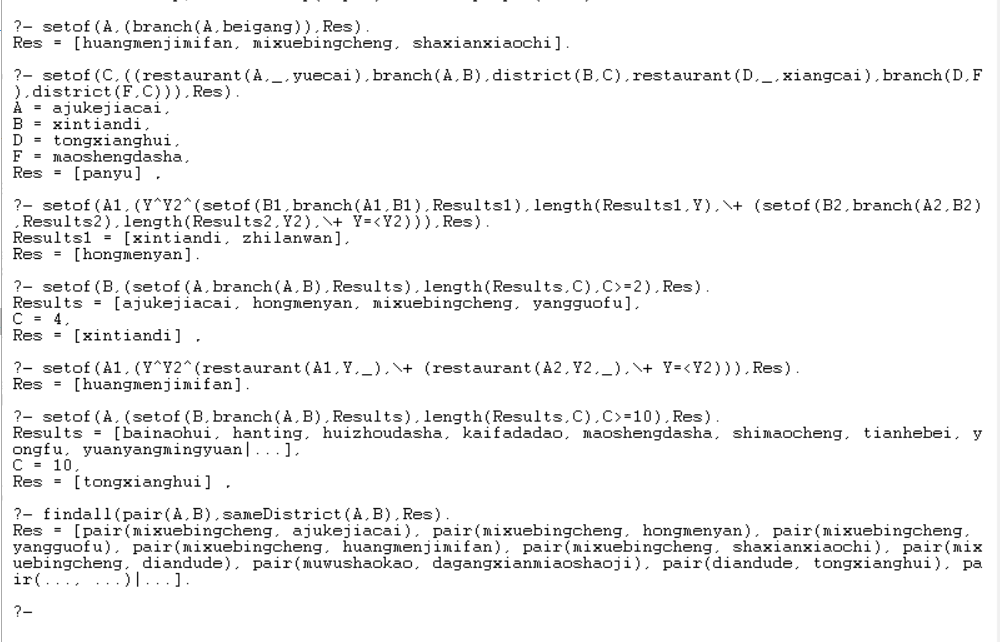
\includegraphics[width=17.3cm]{pic/1_1.png}
\caption{result}
\end{figure}


%\clearpage
%\bibliography{E:/Papers/LiuLab}
%\bibliographystyle{apalike}
\end{document} 
%%% Local Variables:
%%% mode: latex
%%% TeX-master: t
%%% End:
